\documentclass[9pt]{beamer}
\usetheme{Antibes}
\useinnertheme{rectangles}
\useoutertheme{infolines}
\usepackage[utf8]{inputenc}
\usepackage[T1]{fontenc}
\usepackage[ngerman]{babel}

% patch the look of +, = in arev
\usefonttheme{serif} 

\usepackage{arev}
\usepackage{amsmath}
\usepackage{amssymb}
\usepackage{booktabs}

\setbeamertemplate{footline}{%
\begin{beamercolorbox}[ht=3.0ex,dp=1ex]{title in head/foot}
\hfill\footnotesize\insertpagenumber\enspace\enspace\end{beamercolorbox}}

\definecolor{bluegreen1}{rgb}{0.0,0.20,0.28}
\definecolor{bluegreen2}{rgb}{0.0,0.20,0.28}
\setbeamercolor*{palette primary}{fg=white,bg=bluegreen1}
\setbeamercolor*{palette secondary}{fg=white,bg=bluegreen2}
\setbeamercolor*{palette tertiary}{fg=white,bg=bluegreen2}
\setbeamercolor{itemize item}{fg=black}
\setbeamercolor{block title}{bg=bluegreen2}
\newcommand{\modest}[1]{{\small\color{gray}#1}}

\newcommand{\ee}{\mathrm e}
\newcommand{\ui}{\mathrm i}
\newcommand{\real}{\operatorname{Re}}
\newcommand{\imag}{\operatorname{Im}}
\newcommand{\uv}[1]{\underline{#1}}
\newcommand{\bv}[1]{\mathbf{#1}}

\newcommand{\N}{\mathbb N}
\newcommand{\Z}{\mathbb Z}
\newcommand{\Q}{\mathbb Q}
\newcommand{\R}{\mathbb R}
\newcommand{\C}{\mathbb C}

\newcommand{\id}{\operatorname{id}}
\newcommand{\sgn}{\operatorname{sgn}}
\newcommand{\Abb}{\operatorname{Abb}}
\newcommand{\unit}[1]{\mathrm{#1}}
\newcommand{\chem}[1]{\mathrm{#1}}
\newcommand{\strong}[1]{\textsf{\textbf{#1}}}
\newcommand{\defiff}{\quad:\Longleftrightarrow\quad}

\newcommand{\icol}[1]{
  \big(\!\begin{smallmatrix}#1\end{smallmatrix}\!\big)%
}

\newcommand{\parspace}{\vspace{0.8em}}

\usepackage{epsdice}
\newcommand\dice[1]{\vcenter{\hbox{\epsdice{#1}}}}


\title{Was ist Wahrscheinlichkeit?}
\date{}

\begin{document}

\begin{frame}
\maketitle

\vspace{-8em}
\begin{center}
\includegraphics[width=24mm]{img/dices.pdf}
\end{center}

\end{frame}

\begin{frame}[t]
\vspace{4em}
Betrachten wir einen klassischen Spielwürfel.\pause

\vspace{0.8em}
Die unterschiedlichen Ergebnisse, wie ein Wurf ausgehen kann, fassen
wir zur \emph{Ergebnismenge} $\Omega$ zusammen.\pause

\vspace{1.2em}
D.\,h.
\[\Omega := \{\dice{1}, \dice{2}, \dice{3}, \dice{4}, \dice{5}, \dice{6}\}.
\]\pause

\vspace{0.4em}
Kurz
\[\Omega := \{1, 2, 3, 4, 5, 6\}.\]
\end{frame}

\begin{frame}
Die Teilmengen von $\Omega$ nennen wir \emph{Ereignisse}.\pause

\parspace
Das Zufallsexperiment bestehe im Wurf des Würfels.\pause

\begin{definition}
Ein Ereignis $A$ ist beim Zufallsexperiment eingetreten,
wenn das Ergebnis in $A$ liegt.
\end{definition}\pause
Betrachten wir bspw. die Ereignisse
\[A := \{\dice{1},\dice{2}\},\quad B := \{\dice{2},\dice{3}\},\quad C := \{\dice{1}\}.\]
Beim Wurf kam das Ergebnis $\dice{3}$ bei raus.\pause

\parspace
Dann ist $B$ eingetreten, die Ereignisse $A,C$ jedoch nicht.
\end{frame}

\begin{frame}
Die zentrale Frage liegt nun darin, wie es bei einem Ereignis
um die Chance für den Eintritt steht.\pause

\parspace
Ist der Würfel ungezinkt, sollten doch die Chancen zwischen den
sechs Seiten gleichverteilt sein.\pause

\parspace
Zur zahlenmäßigen Erfassung bekommt jedes Ereignis $A$ eine Zahl
$P(A)$ aus dem Intervall $[0,1]$ zugeordnet, die wir
\emph{Wahrscheinlichkeit} nennen, engl. \emph{probability}.\pause

\parspace
Wird das gleiche Experiment sehr oft wiederholt, ist
\[P(A) \approx \frac{\text{Anzahl der Eintritte von $A$}}{\text{Gesamtzahl der Versuche}}.\]
\end{frame}

\begin{frame}[t]
\vspace{6em}
Weil es zwingend zu einem der Ergebnisse kommen muss, ist
\[P(\Omega) = 1.\]\pause
Verteilen wir diese Wahrscheinlichkeit gleichmäßig auf die sechs
elementaren Ereignisse, bringt uns das
\begin{gather*}
P(\{\dice{1}\}) = \tfrac{1}{6},\quad P(\{\dice{2}\}) = \tfrac{1}{6},\quad
P(\{\dice{3}\}) = \tfrac{1}{6},\\
P(\{\dice{4}\}) = \tfrac{1}{6},\quad P(\{\dice{5}\}) = \tfrac{1}{6},\quad
P(\{\dice{6}\}) = \tfrac{1}{6}.\\
\end{gather*}
\end{frame}

\begin{frame}[t]
\vspace{4.6em}
Man spricht von einer \emph{Gleichverteilung}.\pause

\parspace
Die Gestalt einer Verteilung wird sichtbar an ihrer
\emph{Wahrscheinlichkeitsfunktion} $p(\omega):=P(\{\omega\})$.\pause

\begin{center}
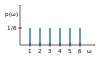
\includegraphics[width=54mm]{img/dice-uniform.pdf}
\end{center}
\end{frame}

\begin{frame}
\begin{center}
\strong{Ermittlung von Wahrscheinlichkeiten}
\end{center}
\end{frame}

\begin{frame}
Wie bestimmt man nun die Warscheinlichkeit beliebiger
Ereignisse wie $\{\dice{1},\dice{2}\}$ oder
$\{\dice{1},\dice{2},\dice{3}\}$?
\end{frame}

\begin{frame}[t]
\vspace{4em}
Wir interpretieren ein Ereignis als eine Fläche und die
Wahrscheinlichkeit als den Flächeninhalt.\\

\vspace{0.8em}
Je größer die Fläche,
desto wahrscheinlicher ist das Ereignis.\pause
\begin{center}
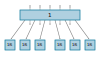
\includegraphics[width=60mm]{img/propability-area.pdf}
\end{center}
\end{frame}

\begin{frame}[t]
\vspace{4em}
Wir sagen, zwei Ereignisse $A,B$ sind disjunkt, wenn sie
leeren Schnitt haben, kurz $A\cap B=\emptyset$. Dies bedeutet, die
Ereignisse besitzen keine gemeinsamen Elemente, bzw. ihre Flächen
überlappen nicht.\pause

\vspace{0.8em}
Unter dieser Prämisse ist der Flächeninhalt der Vereinigung
$A\cup B$ doch die Summe der beiden Teile.\pause{} D.\,h.
\[P(A\cup B) = P(A) + P(B).\qquad (A\cap B=\emptyset)
\]\pause

\vspace{-2em}
\begin{center}
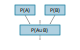
\includegraphics[width=50mm]{img/additivity.pdf}
\end{center}
\end{frame}

\begin{frame}
Liegen zwei Ereignisse vor, die nicht disjunkt sind, z.\,B.
\[A=\{\dice{1},\dice{2}\},\quad B=\{\dice{2},\dice{3}\},\]
dann überlappen die Flächen, und der Flächeninhalt
der Überlappung würde doppelt gezählt.\pause

\vspace{-1em}
\begin{center}
\includegraphics[width=34mm]{img/intersection.pdf}
\end{center}\pause

\vspace{-1em}
Um das zu berichtigen, muss der Flächeninhalt der Überlappung
einmal abgezogen werden.\pause{} Das macht
\[P(A\cup B) = P(A) + P(B) - P(A\cap B).\]
\end{frame}

\begin{frame}
Die Regel liefert
\[P(A) = P(\{\dice{1}\}\cup\{\dice{2}\})
= P(\{\dice{1}\})+P(\{\dice{2}\}) = \tfrac{1}{6}+\tfrac{1}{6}
= \tfrac{2}{6}.\]\pause
Auf die gleiche Art erhält man $P(B)=\tfrac{2}{6}$.\pause

\vspace{0.8em}
Für $A\cup B = \{\dice{1},\dice{2},\dice{3}\}$ ist auf einem Wege
\[P(A\cup B) = P(\{\dice{1}\}) + P(\{\dice{2}\}) + P(\{\dice{3}\})
= \tfrac{1}{6}+\tfrac{1}{6}+\tfrac{1}{6} = \tfrac{1}{2}.\]\pause
Und mit $A\cap B = \{\dice{2}\}$ auf anderem Wege
\[P(A\cup B) = P(A) + P(B) - P(A\cap B)
= \tfrac{2}{6}+\tfrac{2}{6} - \tfrac{1}{6} = \tfrac{1}{2}.\]\pause
Beide Rechenwege führen zum gleichen Ergebnis.
\end{frame}

\begin{frame}
Der erste Rechenweg bietet eine Abkürzung. Die Herleitung dazu
verlangt allerdings die Formulierung in allgemeiner Form.\pause

\parspace
Zunächst zerlegen wir ein Ereignis in dessen elementare
Ereignisse:
\[A = \bigcup_{\omega\in A} \{\omega\}.\]
Z.\,B. ist
\[\{\dice{1},\dice{2},\dice{3}\}
= \{\dice{1}\}\cup\{\dice{2}\}\cup\{\dice{3}\}.
\]\pause
Die elementaren Ereignisse sind alle disjunkt, womit sich die
Vereinigung unter~$P$ -- wie schon bekannt --
in eine Summe verwandelt.\pause

\parspace
Aufgrund der Gleichverteilung besitzt nun jedes elementare Ereignis
die gleiche Wahrscheinlichkeit $\tfrac{1}{|\Omega|}$, wobei mit
$|\Omega|$ die Anzahl der Elemente von $\Omega$ gemeint ist.
\end{frame}

\begin{frame}
Daher gilt
\[P(A) = P(\bigcup_{\omega\in A}\{\omega\})
= \sum_{\omega\in A} P(\{\omega\}) = \sum_{\omega\in A}\tfrac{1}{|\Omega|}
= \tfrac{1}{|\Omega|}\cdot\sum_{\omega\in A} 1 = \tfrac{1}{|\Omega|}\cdot |A|.
\]\pause
\begin{block}{Satz (Laplace-Formel)}
Bei einer Gleichverteilung gilt
\[P(A) = \frac{|A|}{|\Omega|}.\]
\end{block}\pause
Das macht
\[P(\{\dice{1},\dice{2},\dice{3}\}) = \frac{3}{6} = \frac{1}{2}.\]
\end{frame}

\begin{frame}
\begin{center}
\strong{Zufallsgrößen}
\end{center}
\end{frame}

\begin{frame}
Die Frage, wie hoch die Wahrscheinlichkeit für ein gerades Ergebnis
ist, beantwortet wohl jeder sofort intuitiv mit $\tfrac{1}{2}$. Auch
mit der bisher erläuterten Methode geht das, es handelt sich ja
schlicht um das Ereignis $\{\dice{2},\dice{4},\dice{6}\}$.\pause

\parspace
In dieser schlichten Überlegung liegt ein unheimlich tiefgreifendes
Konzept verborgen. Dazu wird »ist gerade« als Funktion
\[X\colon\Omega\to\{0,1\},\quad
X(\omega) := \begin{cases}
1 & \text{wenn $\omega$ gerade ist},\\
0 & \text{sonst}
\end{cases}\]
betrachtet.\pause{} Wertetabelle:
\begin{center}
\begin{tabular}{c|cccccc}
$\omega$ & $\dice{1}$ & $\dice{2}$ & $\dice{3}$ & $\dice{4}$ & $\dice{5}$ & $\dice{6}$\\
\midrule
$X(\omega)$ & 0 & 1 & 0 & 1 & 0 & 1
\end{tabular}
\end{center}
\end{frame}

\begin{frame}[t]
\vspace{3em}
Eine solche Funktion $X\colon\Omega\to\Omega'$ nennt sich
\emph{Zufallsgröße}.\pause

\parspace
Von Belang ist nun, wann ein Ereignis $A'$ auf $\Omega'$ eintritt.
Dafür verantwortlich sind doch genau die Ergebnisse aus $\Omega$,
deren Funktionswert in $A'$ liegt.\pause

\parspace
Die Menge dieser Elemente von $\Omega$ ist das Urbild $X^{-1}(A')$.\pause

\begin{center}
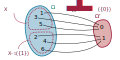
\includegraphics[width=72mm]{img/preimage.pdf}
\end{center}
\end{frame}

\begin{frame}
Demnach ist die Wahrscheinlichkeit für den Eintritt von $A'$ doch
gleich der Wahrscheinlichkeit für den Eintritt des Urbilds.\pause

\parspace
D.\,h.
\[P(A') = P(X^{-1}(A')).\]\pause
Das $P$ auf der linken Seite ist genauer gesagt eine neue Funktion $P_X$.
Man nennt $P_X$ die \emph{Verteilung} der Zufallsgröße $X$.
\end{frame}

\begin{frame}
Damit ist die gesuchte Wahrscheinlichkeit ermittelbar:
\[P_X(\{1\}) = P(X^{-1}(\{1\})) = P(\{\dice{2},\dice{4},\dice{6}\})
 = \tfrac{1}{2}.\]
\end{frame}

\begin{frame}
\strong{Bemerkung.} Zur Angabe der Wahrscheinlichkeit des Urbildes hat
sich\\
im Laufe der Zeit eine ungewohnte Notation entwickelt. So gibt es
die Kurzschreibweisen
\[P(X\in A') := P(X^{-1}(A'))\]
und
\[P(X=x) := P(X^{-1}(\{x\})).\]\pause
Bezüglich einem Ereignis
\begin{align*}A' &= \{a\in\Omega'\mid a\le x\}\\
&= \text{Menge der $a$, für die gilt: $a\le x$}
\end{align*}
gibt es zudem
\[P(X\le x) := P(X^{-1}(A')).\]
\end{frame}

\begin{frame}
Ende.
\vfill\hfill\modest{Juli 2020}\\
\hfill\modest{Creative Commons CC0 1.0}
\end{frame}


\end{document}


